\chapter{Bare Metal Programming}
Bare-Metal Programming (BMP) is a common approach in embedded systems where software runs directly on hardware without requiring an operating system. This method provides direct control over hardware resources, ensuring low latency and high performance. Additionally, debugging techniques are explored to analyze and optimize the code execution.

\section{Vivado}
Vivado is a software developed by AMD, oriented to programming FPGAs, which supports various board and modules. The example project that will be discussed within this chapter is meant only to give an introduction to the Vivado-FPGA programming world, which is way more vast and deeper.
\begin{figure}[h!t!]
	\centering
	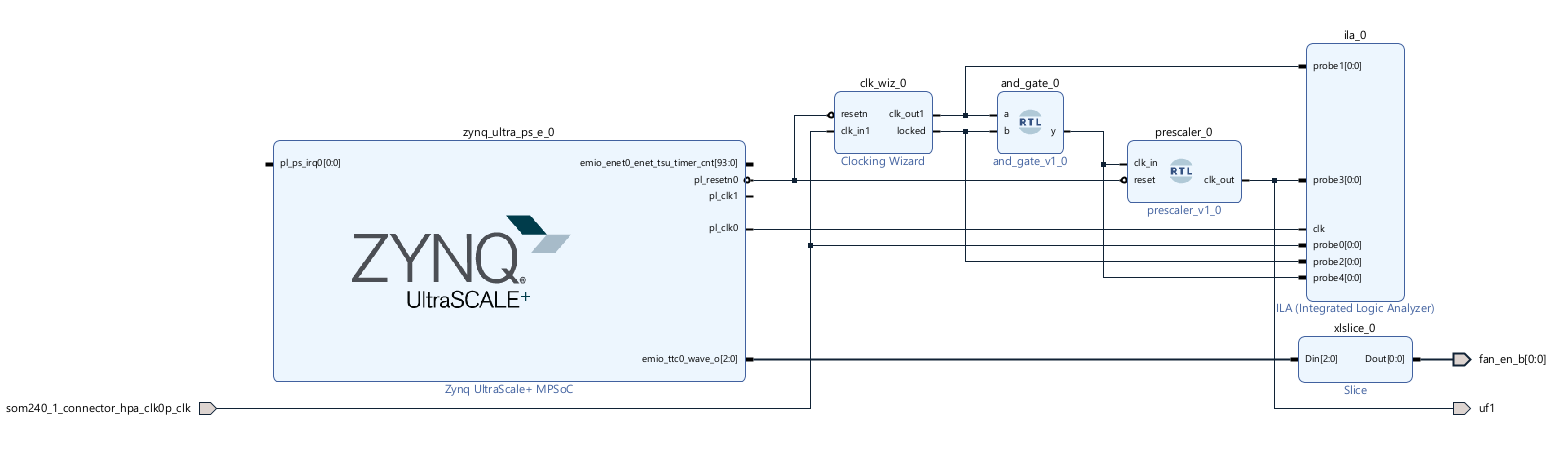
\includegraphics[width=1\textwidth]{images/prj3_1}
	\caption{Block scheme of the Vivado design.}
	\label{fig:prj3_1}
\end{figure}
Figure \ref{fig:prj3_1} presents a simple blinking LED design. In addition to the standard blocks imported from the example on which the design is based, the project includes several additional blocks required for proper functionality. Even though in the design is reported also the system processor block, the procedure will not deepen the Petalinux configuration, topic which will be touched in the next chapter.

\paragraph{Clocking Wizard} The Clocking Wizard is responsible for the generation of a 10 MHz clock source within the project. The IP is imported from the IP list of Vivado, thus no code is available for consultation. However, a block configuration procedure is needed to define the block behavior.

\paragraph{And Gate} The AND gate serves to create a stable clock source for the design by allowing the output only when the clocking wizard's output reaches a stable value. The VHDL implementation is given in the following code:
\vspace{0.1cm}
\begin{lstlisting}[language=VHDL]
library IEEE;
use IEEE.STD_LOGIC_1164.ALL;

entity and_gate is
	Port (a, b : in STD_LOGIC;
		    y : out STD_LOGIC);
end and_gate;

architecture Behavioral of and_gate is
begin
	y <= a and b;
end Behavioral;
\end{lstlisting}

\paragraph{Prescaler} The prescaler is used to further divide the clock frequency of the Clocking Wizard's output. Its output is directly connected to the LED, hence, to be visible, the frequency has to be smaller than few tens of Hz.
\vspace{0.1cm}
\begin{lstlisting}[language=VHDL]
-- Clock Divider
-- Every match, the output signal is toogled
-- The output frequency is given by: f_out = f_in / (2*max_val)

library IEEE;
use IEEE.STD_LOGIC_1164.ALL;
use IEEE.STD_LOGIC_ARITH.ALL;
use IEEE.STD_LOGIC_UNSIGNED.ALL;

entity prescaler is
	Port (clk_in, reset : in STD_LOGIC;
		    clk_out : out STD_LOGIC);
end prescaler;

architecture Behavioral of prescaler is
	constant max_val : integer := 500000;
	signal counter : integer range 0 to max_val-1 := 0;
	signal tmp : std_logic := '1';
begin
	process(clk_in, reset)
	begin
		if reset = '0'
		then
			tmp <= '0';
			counter <= 0;
		else
			if rising_edge(clk_in)
			then
				if counter = max_val-1 -- Counts from 0 to max_val-1
				then
					counter <= 0;
					tmp <= not tmp;
				else
					counter <= counter + 1;
				end if;
			end if;
		end if;
	end process;
clk_out <= tmp;
end Behavioral;
\end{lstlisting}

\paragraph{Integrated Logic Analyzer} This device acts like a digital oscilloscope and allows the displaying of the design internal signal that are connected to the blocks probes.




\subsection{Project creation}
The project was created, as aforementioned, starting from a design example. To create the project, open Vivado main page, click on \textbf{Open Example Project} → \textbf{Next} → \textbf{Kria Starter Kit Design Example} → select the KR260 board → rename the project → \textbf{Default Bitstream} → create the project. From the \textbf{Sources} windows delete the already existent wrapper, while keeping the design. To add the and gate and prescaler design blocks, move to \textbf{Sources} → \textbf{Design Sources} → right-click on this latter one → \textbf{Add Sources}.
\begin{figure}[h!t!]
	\centering
	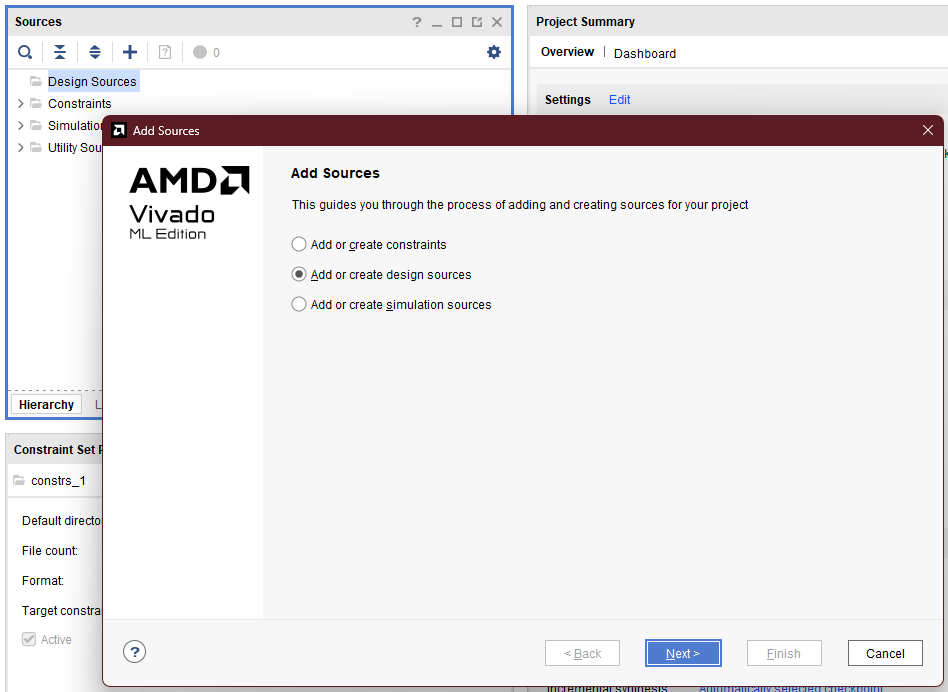
\includegraphics[width=0.8\textwidth]{images/vivado2}
	\caption{Block scheme of the Vivado design.}
	\label{fig:vivado2}
\end{figure}
Select \textbf{Add or create design sources} → \textbf{Next} → \textbf{Create file} → enter the file name → \textbf{Finish}. Once it
is done, a window to configure the inputs and the outputs of the gate should open. Such procedure can be skipped, providing that those information are defined in the description.

The Physical Constraint File (PCF) defines the mapping between the FPGA's internal logic and the physical pins of the development board. It specifies which FPGA pin is connected to which external component, such as LEDs, switches, or communication interfaces. This file is crucial for real-life applications, ensuring that the synthesized design correctly interfaces with the hardware. The process of defining physical constraints follows a procedure similar to the one used for behavioral descriptions (\textbf{Sources} → \textbf{Constraints} → right-click on this latter one → \textbf{Add Sources} → \textbf{Add or create constraints} → \textbf{Next} → \textbf{Create file} → enter the file name → \textbf{Finish}), but instead of describing logic functionality, it focuses on hardware connectivity and signal routing. Proper constraint definition prevents issues like incorrect signal assignment, which could lead to malfunctioning hardware or damage to the FPGA. The code to be written is:
\vspace{0.1cm}
\begin{lstlisting}[language=VHDL]
set_property BITSTREAM.GENERAL.COMPRESS TRUE [current_design]

#User defined pins
set_property PACKAGE_PIN F8 [get_ports {uf1}]
set_property IOSTANDARD LVCMOS18 [get_ports {uf1}]
\end{lstlisting}
\vspace{0.1cm}
A bit of explanation is needed to understand what these few lines of code do. The first line specifies that the bitstream generated for this project will be compressed, which helps reduce the file size, making it more efficient for storage and deployment. The subsequent lines define the physical connections between the FPGA and the hardware components (such as an LED) based on the datasheet of the development board. One line specifies that the LED is connected to a specific pin on the FPGA. This pin is defined as a standard I/O pin with a voltage logic of 1.8V (LVC-MOS18), which means that the pin uses Low Voltage CMOS (LVCMOS) logic at 1.8V to communicate with the LED. These settings ensure the correct functionality of the LED based on the voltage and current requirements of the board and peripheral components.


Under the section of \textbf{IP INTEGRATOR}, click on \textbf{Open Block Design}: a new window will open. Move back to \textbf{Design Sources} → right click on the description file(s) created earlier → \textbf{Add Module to Block Design}. To create a physical connection to the board pins, move the mouse tip on the block pins and type \textbf{Ctrl+T} to add a connection. By clicking on the created pins, a window named \textbf{External Port Properties} should appear. Rename those pins with the name defined in the constraints file. Click on the \textbf{+} sign on the top of the design window, search and add the clocking wizard IP block. Now the design should have the same blocks displayed in Figure \ref{fig:prj3_1}.

\subsection{Block configuration}
It should be now possible to run the automatic connection procedure (green tab on the top of the window). As previously explained, there is the necessity to configure the clocking wizard block (double click on the IP): set the reset to be active low, set the output clock to be the
value that you want (there is, however, a defined range of possible clock frequencies with specific values) and tick the section in which the input and output clock are in-phase. For this example the output frequency is set to be $f_{clk-wiz} = 10MHz$. With the prescaler VHDL code defined above, the clock frequency should be equal to
\begin{equation}
	f_{blink} = \frac{f_{clk-wiz}}{2ma_val} = 10Hz
\end{equation} 
Connect then the and gate, the prescaler and the ILA block as shown in Figure \ref{fig:prj3_1}.



\section{JTAG interface}
The Joint Test Action Group (JTAG) interface is primarily used for testing, debugging and programming FPGA devices during the development. It is a crucial tool in the development flow when working with Xilinx FPGAs, as it allows direct communication between a computer (running Vivado) and the FPGA. Its key features are a) FPGA programming, b)Debugging, c) Boundary-scan testing and d) Accessing internal signals (ILA core).

\subsection{JTAG programming}
To program the FPGA, a file similar to the .hex file used for programming uPs (e.g., ATmega, STM32) is required. However, for FPGA programming, this file is usually in the form of a bitstream file (commonly with extensions like .bit or .bin). The bitstream file contains the configuration data that programs the FPGA, mapping the logical design (created in VHDL, Verilog, or through a high-level tool like Vivado) onto the FPGA's hardware resources. Unlike microcontrollers, where code is executed sequentially, an FPGA is configured with a specific hardware design that defines the logic and behavior of the entire device. Move to the \textbf{PROGRAM AND DEBUG} section and click on \textbf{Generate Bitstream}. Follow the procedure and let the bitstream to be generated. The last step is to effectively program the device. Open the \textbf{Open Hardware Manager} and click on \textbf{Open Target} → \textbf{Auto Connect}, then click on \textbf{Program Device}.

\subsection{JTAG debugging}
After having programmed the FPGA, opene the \textbf{Hardware Manager} and connected the device, Vivado should automatically find the debug-probes file (if not, just re-program the FPGA). Between the various signals, chose one to be referred as trigger and define the trigger event (equal to a value, rising or falling edge...) and run the trigger event for the ILA core. A window similar to that of Figure \ref{fig:prj3_2} should appear.
\begin{figure}[h!t!]
	\centering
	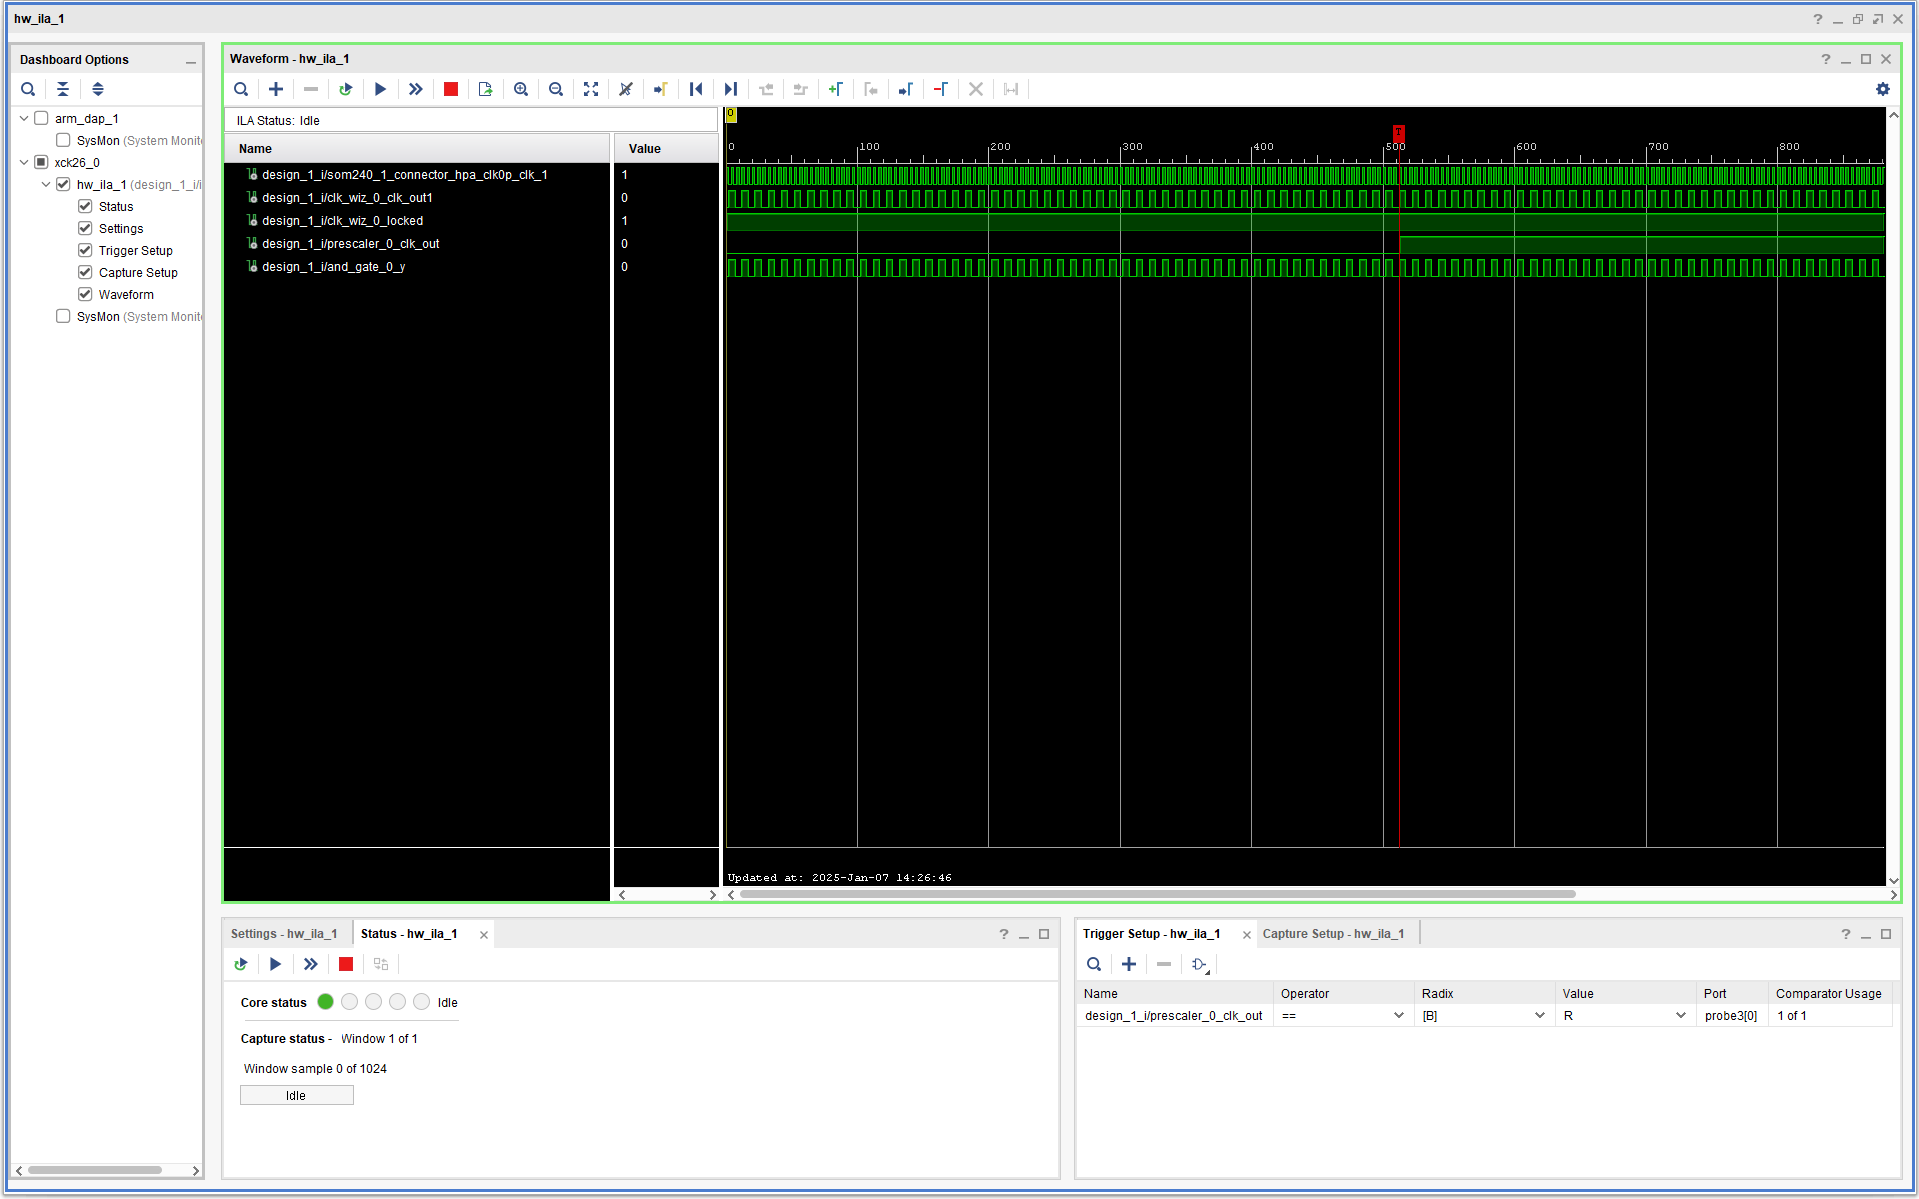
\includegraphics[width=0.8\textwidth]{images/prj3_2}
	\caption{J-tag debugging window.}
	\label{fig:prj3_2}
\end{figure}